%%%%%%%%%%%%%%%%%%%%%%%%%%%%%%%%%%%%%%%%%%%%%%%%%%%%%%%%%%%%%%%%
%%%%%%%%%%%%%%%%%%%%%%%%%%%%%%%%%%%%%%%%%%%%%%%%%%%%%%%%%%%%%%%%
%%%%
%%%% This text file is part of the source of slides for
%%%% `The Art of HPC, vol 1: The Science of Computing'
%%%% by Victor Eijkhout, copyright 2012-2024
%%%%
%%%% slides for performance lecture
%%%%
%%%%%%%%%%%%%%%%%%%%%%%%%%%%%%%%%%%%%%%%%%%%%%%%%%%%%%%%%%%%%%%%
%%%%%%%%%%%%%%%%%%%%%%%%%%%%%%%%%%%%%%%%%%%%%%%%%%%%%%%%%%%%%%%%

\begin{numberedframe}{Justification}
  Programming for performance is an art.

  Here are some examples.
\end{numberedframe}

\begin{numberedframe}{Peak performance}
  \begin{itemize}
  \item Requires all floating point units to be active
  \item Requires all data in L1 cache, or even register
  \item $Rightarrow$~very hard to achieve.
  \end{itemize}
\end{numberedframe}

\begin{numberedframe}{Arithmetic intensity}
  \begin{itemize}
  \item How many operations per word?
  \item Equivalently: reuse factor $=$~ratio between operations and data
  \item Reuse: algorithm vs implementation
  \end{itemize}
\begin{lstlisting}
\end{lstlisting}
\end{numberedframe}

\begin{numberedframe}{Bandwidth-limited operations}
  \begin{itemize}
  \item `Streaming' operations
  \end{itemize}
\cxxverbatimsnippet{bandwidththreads}
\end{numberedframe}

\begin{numberedframe}{Bandwidth measurement}
\includegraphics{../plots/multicore-bandwidth}
  \begin{itemize}
  \item Bandwidth numbers strictly a~posteriori
  \end{itemize}
\end{numberedframe}

\begin{numberedframe}{Cache size effects}
  \begin{itemize}
  \item Basic idea: go many times over a small data set.
  \item The following code is too simple:
  \end{itemize}
\begin{lstlisting}
for (int irepeat=0; irepeat<how_many_repeats; irepeat++) {
  for (int iword=0; iword<cachesize_in_words; iword++)
    memory[iword] += 1.1;
}    
\end{lstlisting}
\end{numberedframe}

\begin{numberedframe}{Random traversal}
  \begin{itemize}
  \item Emulate randomness by pointer chasing
  \end{itemize}
\begin{lstlisting}
// setup
for (int iword=0; iword<cachesize_in_words; iword++)
    memory[iword] = (iword+1) % cachesize_in_words

// use:
ptr = 0
for (int iword=0; iword<cachesize_in_words; iword++)
    ptr = memory[ptr];
\end{lstlisting}
\end{numberedframe}

\begin{numberedframe}{Measurement}
  \includegraphics{../plots/cachesize-bandwidth}
  \begin{itemize}
  \item Explain the step behavior
  \end{itemize}
\end{numberedframe}

\begin{numberedframe}{Associativity}
  \begin{itemize}
  \item Words at certain distance map to the same associativity class
  \item Example: Ice Like has 48KiB cache, 12-way associative
  \item $Rightarrow$~stride 4KiB gives conflict; 12 conflicts can be resolved
  \item Cascade Lake: 8-way associative
  \end{itemize}
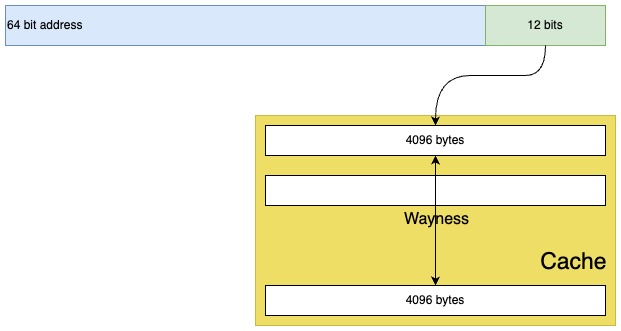
\includegraphics[scale=.6]{../plots/associativity}
\end{numberedframe}

\begin{numberedframe}{Loop tiling}
  \begin{itemize}
  \item Multiple passes over array
  \item Rewrite as by-block
  \item $Rightarrow$~One extra loop level
  \end{itemize}
  \begin{multicols}{2}
\footnotesize
  \begin{lstlisting}
for (n=0; n<10; n++)
  for (i=0; i<100000; i++)
    ... = ...x[i] ...

\end{lstlisting}
\columnbreak
\begin{lstlisting}
bs = ... /* the blocksize */
for (b=0; b<100000/bs; b++)
  for (n=0; n<10; n++)
    for (i=b*bs; i<(b+1)*bs; i++)
      ... = ...x[i] ...
\end{lstlisting}
  \end{multicols}
\end{numberedframe}

\begin{numberedframe}{Example transpose}
\cverbatimsnippet{regulartranspose}
  \begin{itemize}
  \item Does this have any reuse of input or output?
  \end{itemize}
\end{numberedframe}

\begin{numberedframe}{Rewrite}
  \lstset{basicstyle=\scriptsize\ttfamily}
  \cverbatimsnippet{blockedtranspose}
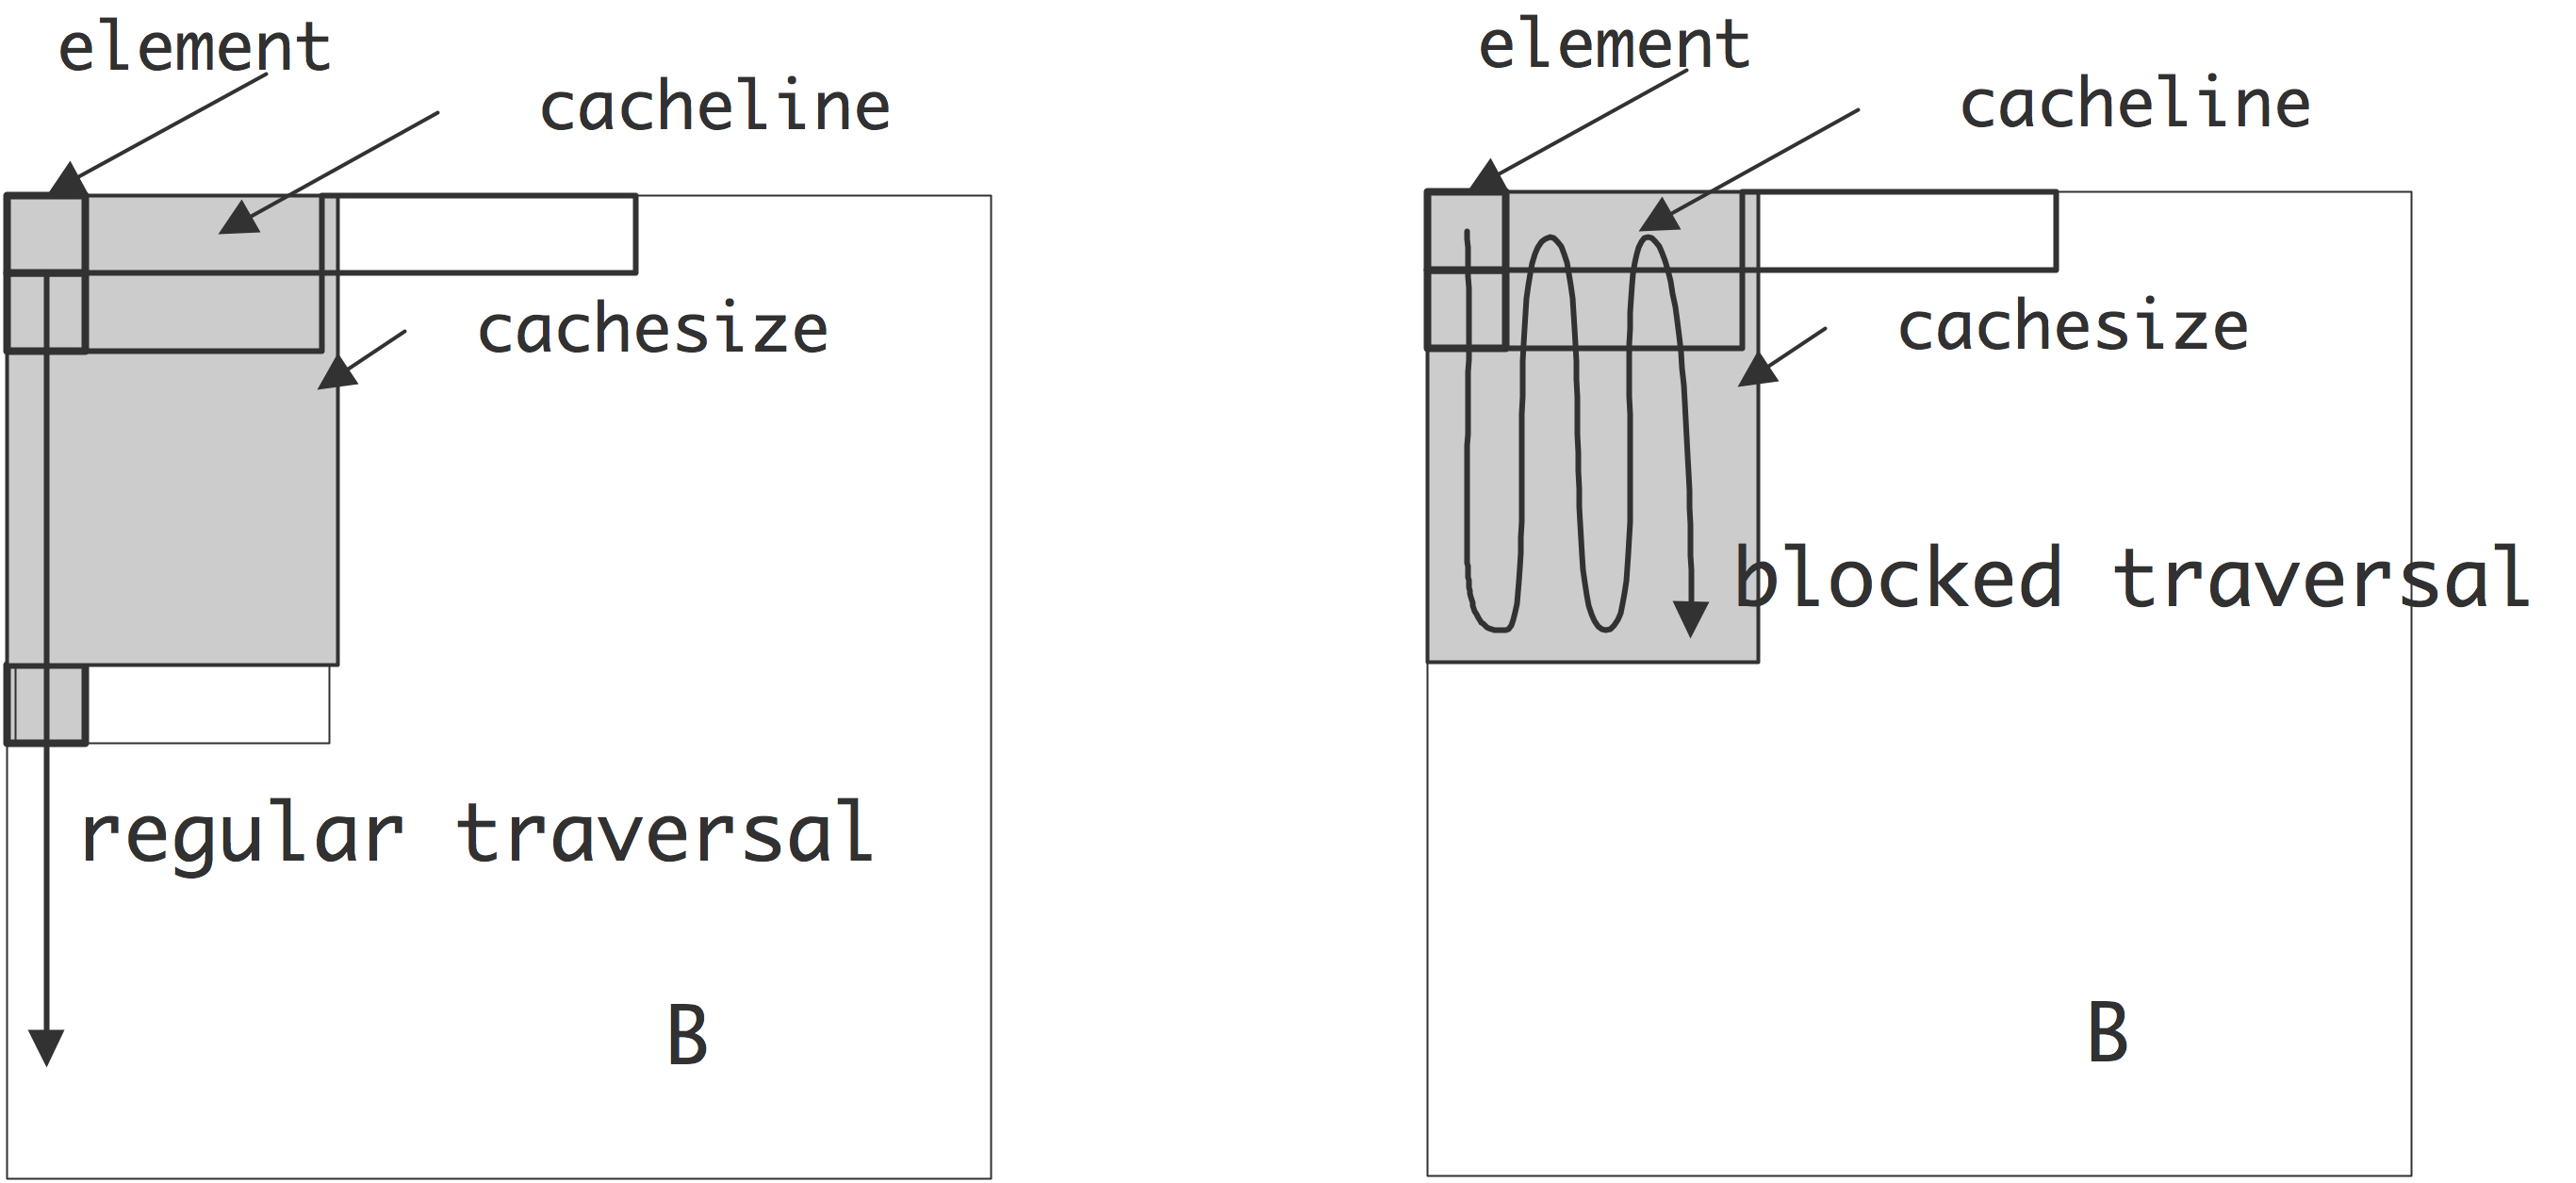
\includegraphics[scale=.12]{blockedtranspose}
\end{numberedframe}

\endinput

\begin{numberedframe}{}
  \begin{itemize}
  \item 
  \end{itemize}
\begin{lstlisting}
\end{lstlisting}
\end{numberedframe}

